\documentclass[14pt,a4paper]{extarticle}
\usepackage[T2A]{fontenc}
\usepackage[utf8]{inputenc}
\usepackage[english,russian]{babel}
\usepackage{lmodern}
\usepackage{geometry}
\usepackage{array}
\usepackage{tabularx}
\usepackage{longtable}
\usepackage{ltablex}
\usepackage{booktabs}
\usepackage{hyperref}
\usepackage{indentfirst}
\usepackage{microtype}
\usepackage{graphicx}
\usepackage{setspace}
\usepackage{listings}
\usepackage{graphicx}
\usepackage{caption}
\usepackage{float}
\usepackage{tocloft}
\usepackage{titlesec}
\usepackage{newtxtext,newtxmath}

\titleformat{\section}        % форматируем \section
  {\normalfont\bfseries}      % стиль: обычный + жирный
  {\thesection.}              % номер секции с точкой
  {2mm}                       % расстояние между номером и текстом
  {}                           % перед заголовком можно добавить что-то
\titlespacing*{\section}{1.5cm}{*3}{*1}  % {отступ слева}{отступ сверху}{отступ снизу}

\captionsetup{justification=centering}
\renewcommand{\ttdefault}{cmtt}
\keepXColumns
\setlength{\parindent}{3em}
\newgeometry{left=2.5cm,right=2.5cm,top=3cm,bottom=2.5cm}

\renewcommand{\contentsname}{\hspace*{4em}{\smallСодержание}}
\setlength{\cftbeforesecskip}{0.5em}
\renewcommand{\cftsecleader}{\cftdotfill{\cftdotsep}}
\renewcommand{\cftsecaftersnum}{.\hspace{2mm}}

\title{Отчёт по дисциплине "Основы предпринимательства"}
\author{Выполнил студент группы М-РИТ-25-1, Станиславчук Сергей}

\begin{document}

\setstretch{1.5}
\noindent
\begin{minipage}[t]{0.01\textwidth}
    \includegraphics{~/programmer/++Programmer/5_1/LSTU.jpg}
\end{minipage}%
\begin{minipage}[c]{1.1\linewidth}
    \centering
    {\small
    МИНИСТЕРСТВО НАУКИ И ВЫСШЕГО ОБРАЗОВАНИЯ РФ \\[1em]
    ФЕДЕРАЛЬНОЕ ГОСУДАРСТВЕННОЕ БЮДЖЕТНОЕ \\
    ОБРАЗОВАТЕЛЬНОЕ УЧРЕЖДЕНИЕ ВЫСШЕГО ОБРАЗОВАНИЯ \\
    «ЛИПЕЦКИЙ ГОСУДАРСТВЕННЫЙ ТЕХНИЧЕСКИЙ УНИВЕРСИТЕТ»
    }
\end{minipage}%

\vspace{3em}

\noindent
\hspace{1em}%
\begin{minipage}[t]{0.8\textwidth}
\textbf{Институт} \hspace{2em} компьютерных наук \\
\textbf{Кафедра} \hspace{2em} автоматизированных систем управления
\end{minipage}


\vspace{6em}

\begin{center}
\textbf{ПРАКТИЧЕСКАЯ РАБОТА №5} \\
по дисциплине \\ <<Основы предпринимательства>>
\end{center}

\vspace{6em}

\noindent
\begin{tabular*}{\textwidth}{@{\extracolsep{\fill}} l c r }
    Студент М-РИТ-25-1 & \makebox[4cm]{\hrulefill} & Станиславчук С.М. \\[2em]
Руководитель & \\
Канд. юр. наук, доцент & \makebox[4cm]{\hrulefill} & Моисеева И.И. \\
\end{tabular*}

\vfill
\begin{center}
    Липецк, 2025
\end{center}

\thispagestyle{empty}

\newpage
\tableofcontents
\newpage

\section{Задание 1}
\begin{sloppypar}
Предприятие производит продукт Х. Величина условно-постоянных затрат
составляет F = 200 млн руб. в год. Максимально возможный объем производства продукта
Х составляет 1 000 единиц в год. Для простоты предположим, что не существует
временного лага между производством и реализацией продукции. Цена единицы
продукции составляет Р=750 тыс. руб. Условно-переменные затраты составляют С=250
тыс. руб. на единицу продукции.
Определите действие операционного рычага, построить график безубыточности.

Решение.

    $V\text{кр} = \frac{F}{(P - C)} = \frac{200 000} {750 - 250} = 400$ шт. - точка безубыточности

\begin{figure}[H]
    \label{fig:pic1}
    \centering
    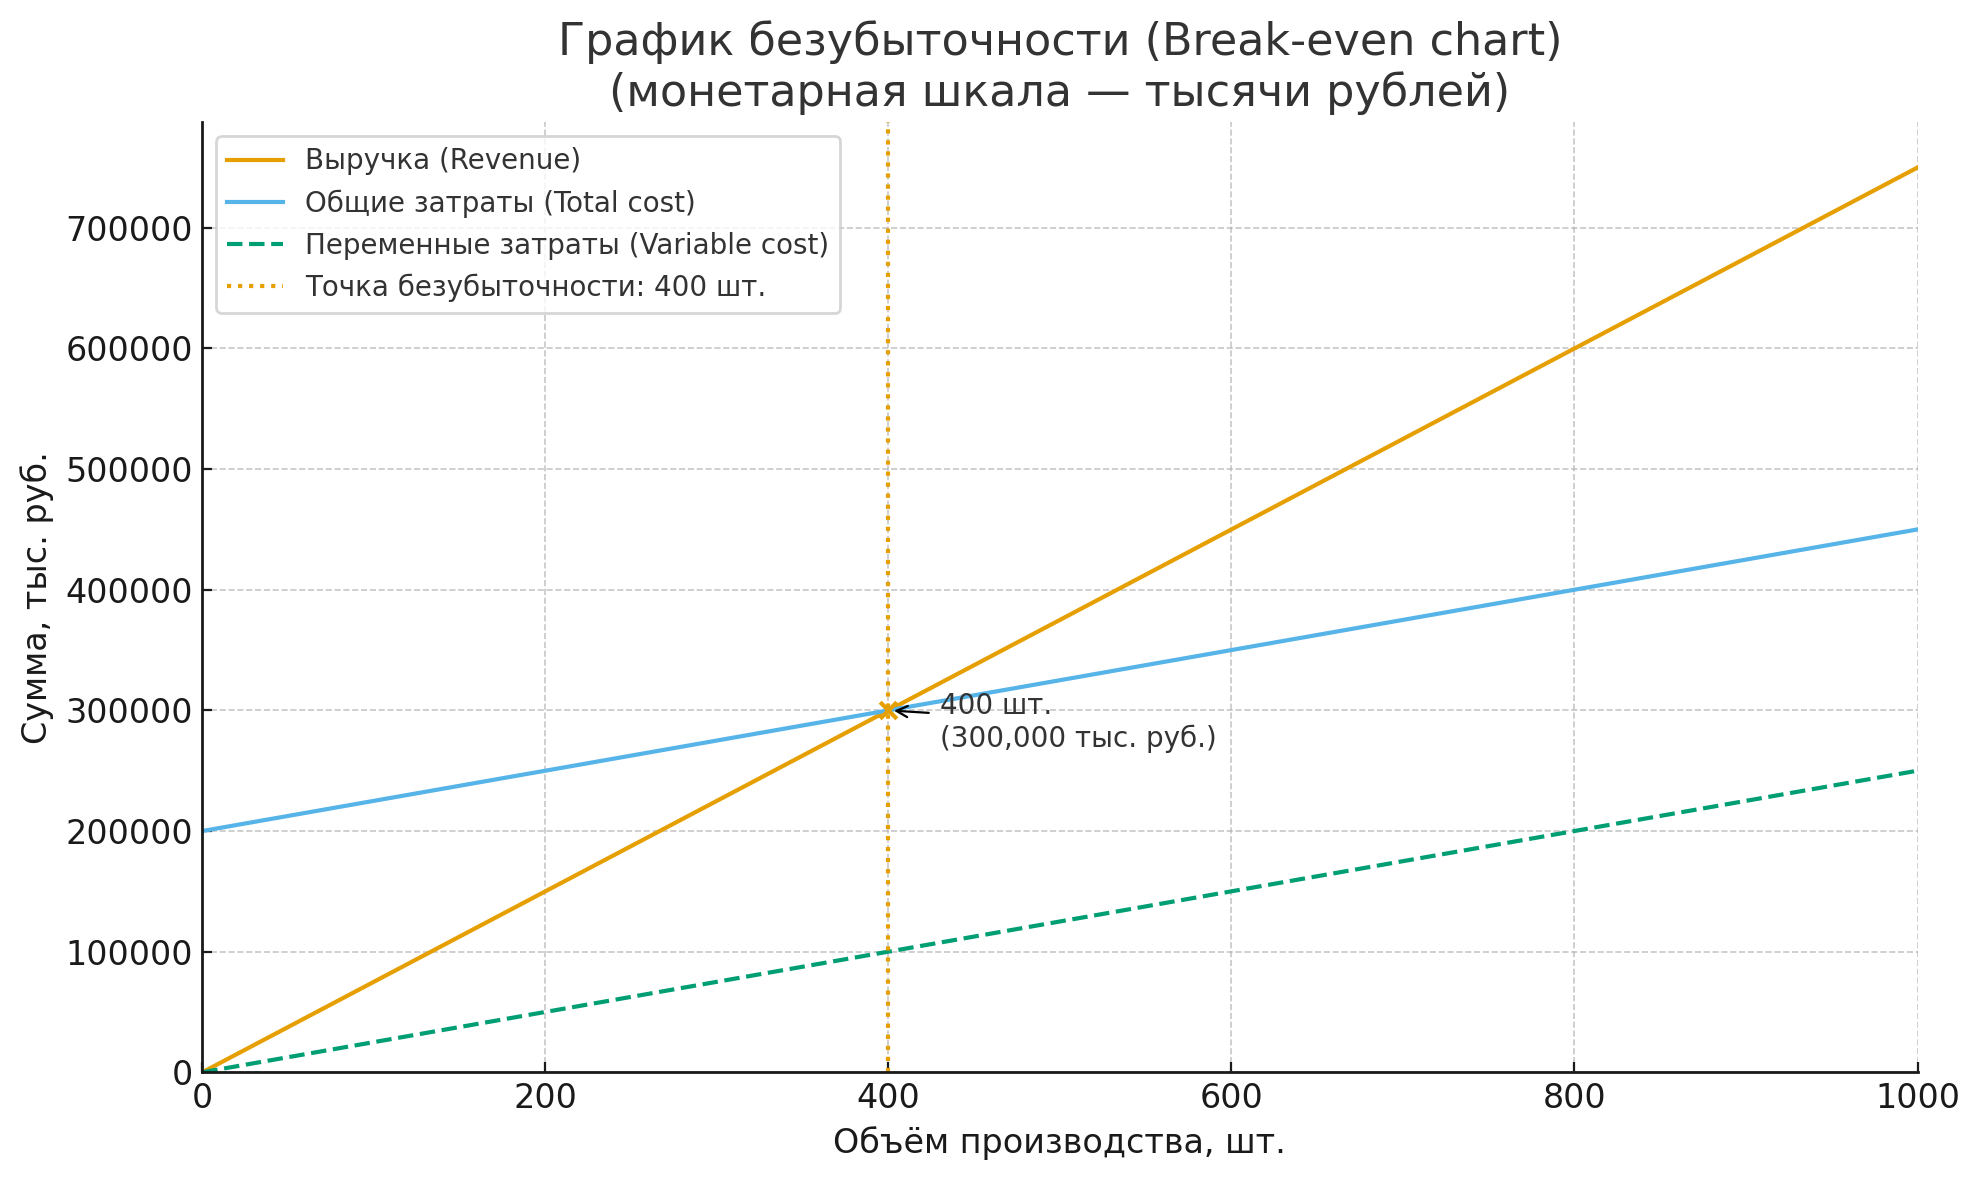
\includegraphics[width=0.78\textwidth]{pic1.png}
    \refstepcounter{figure}
    \caption*{Рисунок \thefigure\ — график безубыточности}
\end{figure}
\end{sloppypar}

\section{Задание 2}
Определите, сколько нужно вложить средств в инвестирование проекта в настоящее
время, чтобы через 7 лет иметь 35 000 ден. ед. при 10\%-й норме доходности инвестиций.

Решение.

$PV = \frac{FV}{(1 + r)^n} = \frac{35 000}{(1 + 0.1)^7} = 17 965.7$ - текущая стоимость

Ответ: 17 966 ден. ед.

\section{Задание 3}
Коммерческая организация планирует через два года приобрести помещение под
офис и склад. Эксперты оценивают будущую стоимость недвижимости в размере 28 млн
руб. По банковским депозитным счетам установлены ставки в размере 22\% с ежегодным
начислением процентов и 20\% с ежеквартальным начислением процентов.
Определите, какую сумму необходимо поместить на банковский депозитный счет,
чтобы через два года получить достаточную сумму для покупки недвижимости.

Решение.

$28 000 000 / (1 + 0.22)^2 = 18 820 000$ => при 22\% годовых. \\
$28 000 000 / (1 + 0.05)^8 = 18 940 000$ => при 20\% годовых, начисление ежеквартально. \\

Ответ: 22\% годовых выгоднее, т.к. требует меньше первоначальных вложений.

\section{Задание 4}

Руководство фирмы намеревается вкладывать деньги в производство новой продукции
с ожидаемой суммой поступлений в размере 116 млн руб. через 4 года. для
обеспечения производства потребуются среднегодовые затраты без амортизационных
отчислений в сумме с налогами и платежами, отнесенными на финансовые
результаты, и налогом на прибыль 5 млн руб. Капитальные вложения в сумме за
весь период инвестирования составляют 60 млн руб. Норма дисконта определена в
размере 11\% в год. Рассчитайте чистый доход от проекта за 4 года.

Решение.

$5 * 4 = 20$ млн.руб. - сумма затрат за 4 года.\\
$NV = FV - (\text{сумма годовых затрат) - капитальные вложения} = 116 - 20 - 60 = 36$ млн.руб. - чистый доход для данного проекта.\\
$NPV = (116 - 20) / (1 + 0.11^4) - 60 = 3.24$ млн.руб.\\
$D = NV - NPV = 36 - 3.24 = 32.76$ млн. руб. - дисконт проекта.\\

Ответ: 32.76 млн.руб.

\section{Задание 5}
Рассчитайте индекс дисконтированной доходности, если чистый дисконтированный
эффект ожидаемого ИП равен 23,71 млн руб. Срок эксплуатации инвестиций
рассчитан на 4 года. Ожидаемая сумма поступлений от проекта равна 116 млн руб.
через 4 года. Общие затраты за весь период эксплуатации инвестиций составят 20
млн руб. Капитальные вложения в сумме за весь период инвестирования равны 60
млн руб. Норма дисконта составляет 11\% в год.

Решение.
\begin{center}
    $PI = \frac{\sum_{t=1}^{n} \frac{R_t - C_t}{(1+r)^t}}{K}$\\
    $PI = 1 + \frac{NPV}{K}$\\
\end{center}
    $ PI = 1 + \frac{23.71}{60} = 1.395 $ - индекс дисконтированной доходности \\

Ответ: 1.395.

\section{Задание 6}
Выберите наиболее доходный способ вложения капитала на 9 лет, если предприятие
может продать на рынке автомобиль по цене 40 ден. ед. и вложить вырученные
деньги в банк под 15\% годовых на условиях сложного процента. В случае
эксплуатации автомобиля через 9 лет остаточная стоимость его составит 10 ден.
ед. Ежегодный доход от использования машины — в среднем 12 ден. ед.

Решение.

$FV = 12 * 9 + 10 = 118$ тыс. руб. - чистый денежный поток через 9 лет при эксплуатации авто. \\
$FV_n = \frac{ PV }{(1 + r)^n}$ \\
$r = 15 / 100 = 0.15$ \\
$FV_n = \frac{40} {(1 + 0.15)^ 9}  = 141$ тыс. руб. - чистый денежный поток через 9 лет при вложении в банк суммы эквивалентной стоимости авто. \\

Ответ: продать автомобиль и вложить деньги в банк будет более доходным вложением капитала.

\section{Задание 7}
Рассчитайте норму прибыли на собственный капитал для двух вариантов при
следующих исходных данных (табл. 1):

\begin{figure}[H]
    \label{fig:pic2}
    \centering
    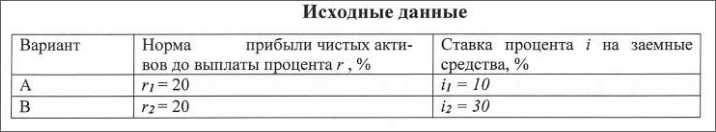
\includegraphics[width=0.78\textwidth]{pic2.png}
    \refstepcounter{figure}
    \caption*{Таблица 1}
\end{figure}

Решение.

$ROE = r + \frac{D}{E} * (r - i)$ \\
$ROE = r + (r - i) = 2r - i$ \\
$ROE_A = 2 * 20 - 10 = 30\%$ \\
$ROE_B = 2 * 20 - 30 = 10\%$ \\

Ответ: 30\% и 10\%

\section{Задание 8}
Определите, сколько нужно вложить средств в инвестирование проекта в настоящее
время, чтобы через 7 лет иметь 35 ден. ед. при 10\%-й норме доходности
инвестиций

Решение.

$PV = 35 / (1 + 0.1)^7 = 35 / (1.1)^7 = 17.96$

Ответ: 17.96 ден. единиц.

\section{Задание 9}
По прогнозу закупка торгового оборудования стоимостью в 8 млн ден.ед. будет
приносить доход в размере 3 млн ден. ед. в год в течение 11 лет. В случае вложения этих
средств в банк предполагается ежегодный доход в размере 12\%.
На основе показателя чистого приведенного эффекта рассчитайте, следует ли
принять проект по закупке и использованию оборудования.

Решение.

$3000 * 11 - 8000 = 25 000$ - прибыль от закупки оборудования \\
$ 8000 * 1.12^{ 11 } = 27828 $ - доход от банковского вклада \\

Ответ: не стоит, прибыльнее вложить деньги в банк.

\section{Задание 10}
Рассчитайте реальную процентную ставку, если длительность шага расчетов равна 1
месяцу, темп инфляции составляет 2 \% в месяц, номинальная процентная ставка — 8 \% в
месяц.

Решение.

$1 + r_{real} = \frac{ 1 + r_{nom} } { 1 + i } = \frac{1 + 0.08}{1+0.02} = 1.0588 = 5.88\%$

Ответ: 5.88\%

\section{Тестирование}
\begin{itemize}
\item 1) а
\item 2) в
\item 3) а, б, в
\item 4) в
\item 5) б
\item 6) в
\item 7) а
\item 8) б
\item 9) в
\item 10) б
\item 11) в
\item 12) б
\item 13) а
\item 14) в
\item 15) а
\end{itemize}

\end{document}
